\documentclass{article}
\usepackage[utf8]{inputenc}
\usepackage{amsmath, amssymb}
\usepackage{graphicx}
\usepackage{geometry}
\usepackage{titlesec}
\usepackage{booktabs}
\usepackage{float}

\geometry{margin=1in}
\newcommand{\sectionbreak}{\clearpage}

\usepackage{hyperref}
\hypersetup{
    colorlinks=true,
    linkcolor=blue,
    filecolor=magenta,      
    urlcolor=blue,}
    
\begin{document}
\newcommand{\calG}{\mathcal{G}}
\title{Physics 742: \\
	Statistical Mechanics \& Condensed Matter\\
	Notes on statistical mechanics and complex networks}
\author{Dion O'Neale}
\maketitle
\newpage
\tableofcontents
\newpage

\section{Thermodynamics - a refresher}
We'll start with a quick overview of some of the important concepts from thermodynamics. Deriving methods for linking these macroscopic concepts to the microscopic state of a system is the original motivation behind much of statistical mechanics. This section will also recap some content from 315/334.

\subsection{Macroscopic laws of thermodynamics}
In thermodynamics we study a system --- the part of the world that we are interested in --- that is separated from its surroundings --- the rest of the universe --- by some boundary.


A \textit{thermodynamic system} is a macroscopic system whose behaviour is identified thanks to a small and finite number of quantities—the thermodynamic properties. If the state of a thermodynamic system can be fully characterized by the values of the thermodynamic variables, and if these values are invariant over time, one says that it is in a state of \textit{thermodynamic equilibrium}. There are many variables which help characterise a macroscopic system, but only a few are actually important. These variables are not independent, and are related to each other with an \textit{equation of state}. An equation of state guarantees that any partial derivatives (which we will see later) are not independent or random, but have mathematical and physical meaning.


For example: the \textit{ideal gas law}
\begin{align*}
pV &= nRT \\
pV &= Nk_{B}T
\end{align*}
can be written an equation of state,
\begin{align*}
p &= f(\rho, T) \\
p &= f(V, N, T)
\end{align*}
where $f()$ is a function to be determined experimentally or with statistical mechanics.

We typically classify systems into three types based on the properties of walls that define the system boundary:
\begin{itemize}
\item {\bf Adiabatic walls/isolated system:} no energy or matter is transferred in or out of the system.
\item {\bf Diathermal walls/closed system:} no matter can be transferred in or out of the system but heat can flow through the walls.
\item {\bf (Semi-)permeable walls/open system:}  in addition to heat, one or more chemical species can be transferred through the walls. 
\end{itemize}
\begin{figure}[H]
	\centering
	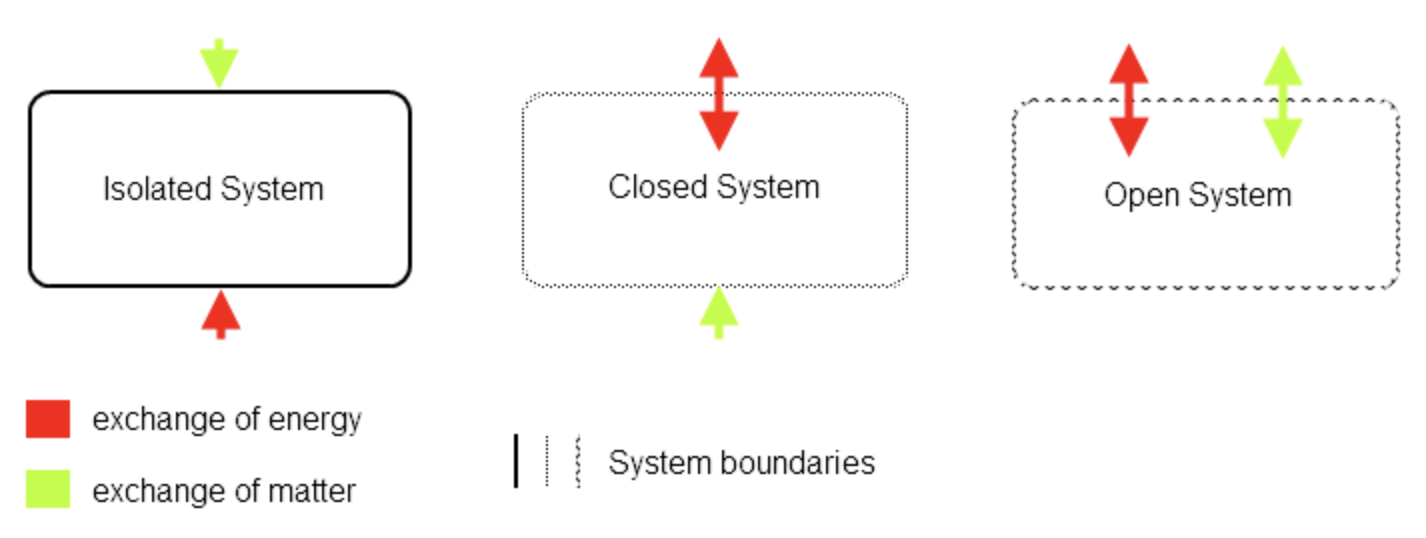
\includegraphics[scale=0.5]{systems}
	\caption{Types of systems, illustrated}
\end{figure}

\subsection*{The four laws of thermodynamics}
Only four laws are required to construct the relationships that control much of classical thermodynamics. Theses are, in brief:
\begin{itemize}
\item {\bf Zeroth law} Defines temperature and thermal equilibrium. 
\item {\bf First law} Formulates the principle of conservation of energy for thermodynamic systems, heat/work are forms of energy; energy is conserved.
\item {\bf Second law} Entropy increases and systems involve towards equilibrium; heat spontaneously flows from high to low temperatures.
\item {\bf Third law} The absolute zero of temperature is not attainable and entropy $\rightarrow$ constant as $T \rightarrow 0$.
\end{itemize}


We'll look the first two laws in a bit more detail and then make use of the second law to derive some familiar properties of heat.

\subsection{The zeroth law:}
If two systems are each in thermal equilibrium with a third system, then they are also in thermal equilibrium with each other. This implies that they have some property in common. We call this property \emph{temperature}. (In the language of mathematics we would say that thermal equilibrium is a transitive property.)

It is worth noting that thermal equilibrium is not the same as thermodynamic equilibrium. For the latter we also need mechanical equilibrium ($p_1=p_2$ --- there are no unbalanced forces) and chemical equilibrium ($\mu_1=\mu_2$ --- equal rates of reaction).

\subsection{The first law}
Heat and work are both forms of energy. The first law of thermodynamics says that energy remains constant for a (collection of) system(s) isolated from their surroundings. We denote work done \emph{on} the system by the surroundings as $W>0$, similarly, heat supplied to the system is denoted $Q>0$. The opposite sign convention holds when it is by the system. Work is path dependent, i.e. it does not only depend on the initial and final states of the system.

When considering the change in energy $\Delta E$ of a system it is necessary to consider both work and heat. For example, if system $A$ gains energy from system $B$, $\Delta E_A = -\Delta E_B \implies \Delta E_A + \Delta E_B =0$. Since, in general, $\Delta E_A\neq W_{B\rightarrow A}$ there will also be a heat flow $Q_{B\rightarrow A}$, due to a temperature difference between systems $A$ and $B$.
So,
$$\Delta E_A = W_{B\rightarrow A} + Q_{B\rightarrow A}$$
$$\Delta E_B = W_{A\rightarrow B} + Q_{A\rightarrow B}.$$

Energy conservation gives 
$$\underbrace{(W_{A\rightarrow B}+W_{B\rightarrow A})}_{\text{Work done by the composite system}} + \underbrace{(Q_{A\rightarrow B}+Q_{B\rightarrow A})}_{\text{Heat flow in the composite system}} = 0$$

In an isolated system the first law gives a sort of balance sheet for energy:
$W_{A\rightarrow B}+W_{B\rightarrow A} = 0$ and $Q_{A\rightarrow B}+Q_{B\rightarrow A}$.

% Revision: Adiabatic work and heat flow. Path dependence of work.
% You may want to incorporate the relevant content about the above concepts into this document.

Suppose work $dW = -p dV$ is done on a closed system and heat is also introduced, but thermodynamic equilibrium is maintained. Then, the change in the internal energy $U$ is $\text{d}U = \text{d}W + \text{d}Q$.


If work is done adiabatically (no energy or matter transfer), then entropy $S$ is constant, so $\text{d}Q = T \text{d}S = 0$. Therefore, $\text{d}U = \text{d}W = -p \text{d}V$.


\textit{When N is constant:} If heat is introduced with no change in volume or other such variable, $\text{d}W = 0$ so $\text{d}U = \text{d}Q = T \text{d}S$.


\textit{When N is not constant:} If heat is introduced with no change in volume or other such variable, $\text{d}W = 0$ so $\text{d}U = \text{d}Q = \mu \text{d}N$.

\subsection{The second law}
The approach to equilibrium has to be characterized by an entropy that increases steadily up to the asymptotic value corresponding to equilibrium. This defines an \textit{irreversible process}.


In a \textit{reversible} process with $\text{d}W = 0$ the entropy necessarily remains fixed at whatever maximal value it had.


Heat flows from hot to cold. Systems in thermal contact will experience this until the temperatures are equal.


If particles can flow from one system to another, they do so with chemical potential from high to low until equal.

\subsection{Internal energy}
The \emph{internal energy} of a system is the energy associated with the internal degrees of freedom of the system. This includes energy that might come from the motion of particles within the system, along with energy due to internal degrees of freedom that might be associated with the molecules that comprise those particles, for example rotational and vibrational degrees of freedom. 

The equation of state for internal energy is often written as $E = E(S,V,N)$ where $S$ is entropy, $V$ is the volume of the system and $N$ is the number of particles. (Note - all of these are extensive variables.)
Looking at the first of these, we can calculate the total derivative of the $E$. We get
$$
	\mathrm{d}E = \frac{\partial E}{\partial S}\mathrm{d}S +  \frac{\partial E}{\partial V}\mathrm{d}V +  \frac{\partial E}{\partial N}\mathrm{d}N.  
$$

The partial derivatives above must be physically relevant. We identify these as 
$$
T =  \frac{\partial E}{\partial S}, \quad p = -\frac{\partial E}{\partial V},\quad \mbox{and}  \quad \mu = \frac{\partial E}{\partial N};
$$ 
temperature, pressure and chemical potential, respectively. (Note the sign on the term for pressure.) This also suggests that we could write the equation of state for internal energy using the intensive variables that we found as the dual variables of $S$ and $V$; namely $E = E(T,p,N)$.

\subsection{Intensive and extensive variables}

\emph{Intensive} variables control the state of a system but are independent of the system size. For example: temperature $T$, pressure $p$, density $\rho$, chemical potential $\mu$

\emph{Extensive}, or additive, variables are proportionate to the size of a system (i.e. they depend on $N$). For example: energy $E$, entropy $S$, heat capacity $C$, particle number $N$, volume $V$.
One important extensive variable is the entropy (or disorder) of a system. As we just showed above, entropy is related to temperature by the internal energy $E$.

It is often helpful to think of intensive and extensive variables as coming in dual pairs with the intensive variable being the derivative of the internal energy with respect to the corresponding extensive variable given all other extensive variables are held constant. For example, $T = \frac{\partial E}{\partial S}\vert_{V,N}$.

Given two systems 1 and 2, an extensive variable for the composite system $1\cup2$ can be found by simply adding the individual extensive variables. For example, $N_{1\cup2} = N_1 + N_2$, $V_{1\cup2} = V_1 + V_2$, $E_{1\cup2} = E_1 + E_2$ ($E$ = internal energy). But this assumption clearly depends on the structural details of the interface. Imagine the oil-water interface in an emulsion like mayonnaise --- in this case the ratio  $\frac{E_{int}}{E_1+E_2}$ is more like $\mathcal{O}(1)$.
Similarly, if there are significant long range interactions, it may not be true that we can treat the extensive variables as being truly additive.
\begin{figure}[H]
	\begin{center}
		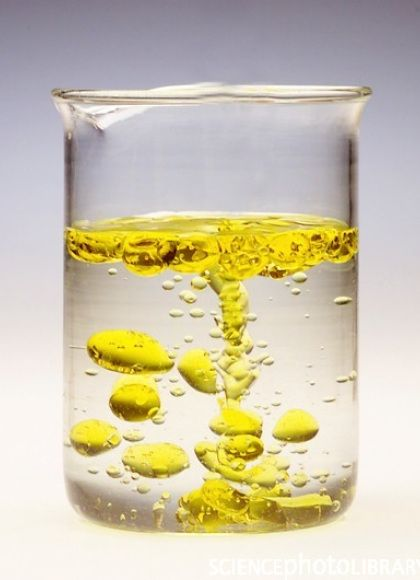
\includegraphics[width=0.2\textwidth]{oilwater}
	\end{center}
	\caption{Oil-water interface}
\end{figure}
The internal energy is not entirely an extensive variable. Since there is often an interaction term between the two systems at the interface. i.e. $E_{1\cup2} = E_1+E_2+E_{int}$. Since $E_{int}$ depends on the interface between the two systems it scales like an area as a function of system size, while $E_1$ and $E_2$ will scale like a volume, so typically $\frac{E_{int}}{E_1+E_2}\rightarrow0$ as the system size gets big. For example, an oil water interface.

\subsection{Heat capacity:}
Heat flowing into a system causes a change in temperature (except in the case of phase transitions). The amount of change in temperature for a given about of heat is the \emph{heat capacity} of the system. The heat capacity of a system depends, in part on the experimental conditions of the system under consideration. Two important cases are constant volume and constant pressure.

For constant volume we have
$$C_V = \frac{\delta Q}{dT}\bigg\vert_V$$
and similarly, for constant pressure,
$$C_p = \frac{\delta Q}{dT}\bigg\vert_p.$$

The first law of thermodynamics (conservation of energy) implies that $\delta Q = dE - \delta W = dE + pdV$  (since $W = Fdx$ and $F=p\times Area \implies W = pdV$). So, since $dV=0$ for constant volume,
$$
	C_V = \frac{\delta Q}{\partial T}\bigg\vert_{V} = \frac{\partial E}{\partial T}\bigg\vert_{V}.
$$


In the constant pressure case 
$$
	C_p = \frac{\delta Q}{dT}\vert_{p} = \frac{\partial E}{\partial T}\vert_{p} + p\frac{\partial V}{\partial T}\vert_{p}.
$$

If we have constant pressure with a change in heat, it implies that there is a change in volume. We define the \emph{volumetric thermal expansivity} as $\alpha_p = \frac{1}{V}\frac{\partial V}{\partial T}\vert_{p}$ and hence $V\alpha_p =\frac{\partial V}{\partial T}\vert_{p}$.

We can now write $C_p = \frac{\partial E}{\partial T}\vert_{p} + \alpha_p pV$. 


We can also find an expression for $C_p$ without resorting to introducing thermal expansivity. Constant pressure implies that $\mathrm{d}(pV)=p\mathrm{d}V$ so that $\delta Q = dE - dW = dE +pdV = d(E+pV)$. We define the composite quantity $E+pV$ as \emph{enthalpy}, $H$.

The infinitesimal for enthalpy is $dH = \underbrace{dE +pdV}_{\delta Q}+ Vdp = \delta Q + Vdp\vert_{p}$. In the constant pressure case, the last term is zero, so we get 
$$
	C_p = \frac{\delta Q}{\partial T}\bigg\vert_{p} = \frac{\partial H}{\partial T}\bigg\vert_{p}. 
$$

% This would be a good place to recall some of the other important thermodynamic quantities and to list the ones that have already been introduced.
% E.g. Entropy, enthalpy, Gibbs/Helmholtz free energy, and some important relationships that can be derived from each of the (the various partial derivatives)

\subsection{Important thermodynamic quantities}

\textit{Entropy} is discussed in section 1.10.


\textit{Enthalpy} $H$ governs the equilibrium of adiabatic processes that occur while pressure is
constant. Among all states that have the same entropy and pressure values, the state of equilibrium is the one that corresponds to the minimum value of enthalpy. Enthalpy is important for chemical reactions in open systems. If a system relaxes toward equilibrium while the pressure is kept constant, the maximum heat that can be produced by the system is equal to its variation in enthalpy. For this reason, enthalpy it is also called free heat.
\begin{align*}
	H(S, p, ..., X_{r}) &= E + pV
\end{align*}

Among all states that have the same temperature and pressure values, the state of equilibrium is that in which the \textit{Gibbs free energy} $G$ assumes the minimum value.
\begin{align*}
	G(T, p, ..., X_{r})  &= E - TS + pV
\end{align*}

The value of the \textit{Helmholtz free energy} $F$ is minimal for the equilibrium state among all virtual states at the given temperature T.
\begin{align*}
	F(T, X) &= E(S(T, X), X) - TS(T, X)
\end{align*}


\subsection{The fundamental hypothesis of thermodynamics}
It is possible to characterise the state of a thermodynamic system by specifying the values of a set of extensive variables.

\subsection{The central problem of thermodynamics}
Given the initial state of equilibrium for several thermodynamic systems that are allowed to interact, we want to be able to determine the final thermodynamic state of equilibrium. The boundaries of the systems --- adiabatic, closed, open --- determine the types of interactions that are allowed, while the four laws of thermodynamics (and the first and second law in particular) determine how the composite system evolves. We want to be able to describe a final thermodynamic equilibrium state from amongst the space of all possible states for the composite system.

Entropy plays a special role in this problem due to the entropy postulate --- the second law of thermodynamics.

\subsubsection*{The entropy postulate}
There exists a function $S$ of the extensive variables $X_1,X_2,\ldots,X_r$, called the entropy, that assumes a maximum value for a state of equilibrium among the space of possible states.

Entropy has the following properties:
\begin{enumerate}
\item Extensivity: If 1 and 2 are thermodynamic systems then $S_{1\cup2}=S_1+S_2$.

\item Convexity: If $X^1=(X_0^1,X_1^1,\ldots,X_r^1)$ and  $X^2=(X_0^2,X_1^2,\ldots,X_r^2)$ are two thermodynamic states of the same system then for $0\leq\alpha\leq1$
$$
	S((1-\alpha)X^1+\alpha X^2)\geq (1-\alpha)S(X^1)+\alpha S(X^2). 
$$
That is, the entropy of a linear combination of states for a single system is greater than or equal to the same linear combination of entropies of the individual states.
A consequence of this is that if we take derivatives with respect to $\alpha$  and then evaluate at $\alpha=0$ we get
$$
	\mbox{LHS:} \quad\frac{\partial}{\partial \alpha} S((1-\alpha)X^1+\alpha X^2) = \sum_{i=0}^r\frac{\partial S}{\partial X_i}(X_i^2-X_i^1)
$$
and
$$
	\mbox{RHS:} \quad\frac{\partial}{\partial \alpha} \left[ (1-\alpha)S(X^1)+\alpha S(X^2) \right] = S(X^2)-S(X^1).
$$

$$ \mbox{Hence,}~~ \sum_{i=0}^r\frac{\partial S}{\partial X_i}(X_i^2-X_i^1)\geq  S(X^2)-S(X^1).$$
Mathematically, this means that the entropy surface (as a function of the other extensive variables) is always below the tangent plane of a point on the surface.

\item Monotonicity: $S(E,X_1,\ldots,X_r)$ is a monotonically increasing function of the internal energy $E$. That is, $\frac{\partial S}{\partial E}\vert_{X_1,\ldots,X_r} = \frac{1}{T}>0$.
\end{enumerate}

Using these three properties, it is possible to find the final equilibrium thermodynamic state amongst the space of possible states of a system. The equilibrium state is the state with maximum entropy that satisfies the constraints on the system.

An example: Consider two closed systems, 1 and 2, in thermal contact such that they can exchange energy, but nothing else (i.e. no other extensive quantities change). The space of possible states is defined by 
$$E^1+E^2 = X_0^1+X_0^2 = E = \text{const.}$$
$$X_i^1 = \text{const.}\quad i=1,2,\ldots,r$$
$$X_i^2 = \text{const.}\quad i=1,2,\ldots,r.$$
We want to find the maximum of $S$ as a function of $E^1$ (we could just as well use $E^2$). Start by taking the derivative of $S$.

\begin{eqnarray*}
	\frac{\partial S}{\partial E^1} &=& \frac{\partial}{\partial E^1}\left(S^1(E^1,X_1^1,X_2^1,\ldots,X_r^1) + S^2(\underbrace{E-E^1}_{E=E^1+E^2},X_1^2,X_2^2,\ldots,X_r^2) \right)\\
	 &=& \frac{\partial S^1}{\partial E^1}\bigg\vert_{E^1} -  \frac{\partial S^2}{\partial E^2}\bigg\vert_{E^2=E-E^1}.
\end{eqnarray*}

For $E^1$ at equilibrium we will write $E^1_{eq}$ (sim. for $E^2$). Then to maximise $S$ we must have
$$
	\frac{\partial S}{\partial E^1}\bigg\vert_{E^1_{eq}} = \frac{\partial S^1}{\partial E^1}\bigg\vert_{E^1_{eq}} - \frac{\partial S^2}{\partial E^2}\bigg\vert_{E-E^1_{eq}}=0
$$
hence
$$
	\frac{\partial S^1}{\partial E^1}\vert_{E^1_{eq}} = \frac{\partial S^2}{\partial E^2}\vert_{E_{eq}^2}.
$$ We already have our first result --- the equilibrium state of the composite system is the one where the change in entropy of the two systems, with respect to, $E$ is equal. Since $\frac{\partial E}{\partial S} = \frac{1}{T}$ (by monotonicity) this means that the equilibrium occurs when the temperatures of the two sub-systems are equal.

Where does the heat flow to in the system in order to reach this equilibrium? The system started in an initial state with $E = E^1_{in}+E^2_{in}$. Since entropy increases to reach the maximum value at equilibrium we have 
$$
	S^1(E^1_{eq}) + S^2(E^2_{eq}) \geq S^1(E^1_{in}) + S^2(E^2_{in}),
$$ 
so,
$$ 
	S^1(E^1_{in}) - S^1(E^1_{eq})  +  S^2(E^2_{in}) - S^2(E^2_{eq})\geq 0.
$$

The convexity property of entropy means that both systems  1 and 2 have 
$$
	\frac{\partial S}{\partial E}\vert_{E_{in}}(E_{eq}-E_{in})\geq S(E_{eq})-S(E_{in})
$$ 
and from the previous expression, the RHS of this inequality is bounded below by zero so we have
$$
	\frac{\partial S^1}{\partial E^1}\bigg\vert_{E^1_{in}}(E_{eq}^1-E_{in}^1) + \frac{\partial S^2}{\partial E^2}\bigg\vert_{E^2_{in}}(\underbrace{E-E_{eq}^1}_{=E^2_{eq}}-E_{in}^2)\geq0
$$

But $E$ is conserved so $E=E^1_{in}+E^2_{in}$ and hence $E-E^1_{eq}-E^2_{in} = -(E^1_{eq}-E^1_{in})$. Therefore
$$
	\left[\frac{\partial S^1}{\partial E^1}\bigg\vert_{E^1_{in}} - \frac{\partial S^2}{\partial E^2}\bigg\vert_{E^2_{in}}\right]\left(E^1_{eq}-E^1_{in}\right)\geq 0.
$$

This implies that energy flows to the  system with higher $\frac{\partial S}{\partial E}$ and since $\frac{\partial S}{\partial E}= \frac{1}{T}$ this means that energy flows into the system with lowest temperature, until the temperatures are equal.

\subsection{Recommended reading}
\begin{itemize}
	\item Sections 2.1 - 2.10 of \emph{Statistical Mechanics in a Nutshell}
\end{itemize}



\section{Student notes from assignment one}




\end{document}
